
\newpage
\section{Casos de uso}
El la siguiente sección se definen y describen los actores, funciones y escenarios, explicando su funcionalidad e interacción con la aplicación.\par
\vspace{5mm}
\begin{figure}[h!]
	\centering
	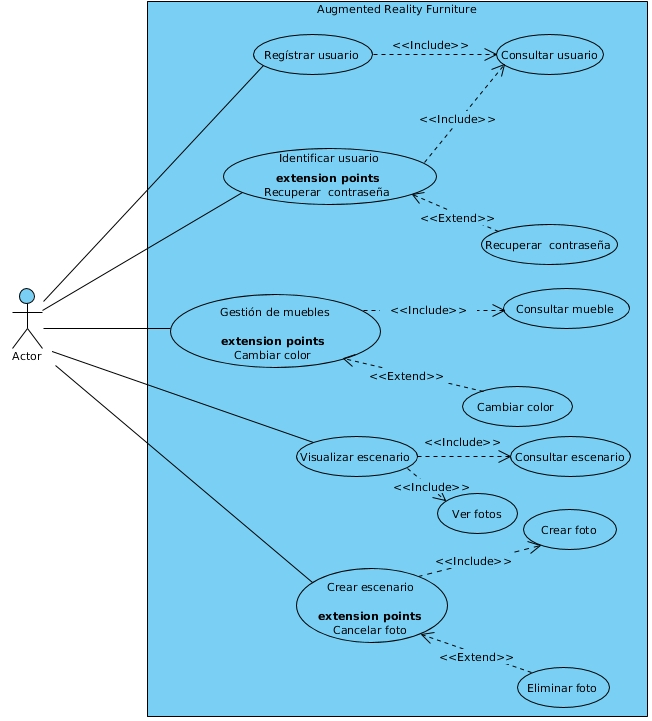
\includegraphics[width=15cm,height=17cm]{imagenes/analisis/casosDeUso.jpg}
	\caption{Casos de uso.}
	\label{fig:analogo}
\end{figure}  
\newpage

\subsection{CU1. Iniciar sesión}\par
Es el escenario de autenticación y acceso de usuario a la aplicación. 
\begin{itemize}
	\item El usuario introduce su usuario y contraseña en los campos de textos mostrados.
	\item El usuario selecciona el botón "Iniciar sesión".
	\item Si algún dato es omitido o está mal escrito (por ejemplo, si el campo "usuario" no tiene la estructura de un email) se mostrará un mensaje en pantalla notificando el error.
	\item De no haber errores, el sistema consulta en la base de datos si se encuentra un registro con los datos ingresados por el usuario.
	\item Si encuentra una coincidencia, se muestra el menú principal donde el usuario puede visualizar sus escenarios y proyectos. Si no se encuentra una coincidencia, se muestra un mensaje en pantalla diciendo que los datos ingresados son incorrectos, y la pantalla mostrada seguirá siendo el Login mientras la autenticación no sea exitosa.
\end{itemize}

\subsection{CU2. Registrar cuenta} \par
Es el escenario donde un usuario registra una nueva cuenta para poder tener acceso al sistema.
\begin{itemize}
	\item En la pantalla inicial, el usuario selecciona el botón "Registrar".
	\item Se mostrará una pantalla con un pequeño formulario donde el usuario ingresará sus datos como son: nombre, email y contraseña. La contraseña debe cumplir con la BR2. También habrá un campo adicional donde deberá introducir de nuevo la contraseña para verificar que el usuario la escribió como la pensó inicialmente.
	\item Tras haber llenado esos campos el usuario selecciona el botón "Registrar cuenta".
	\item Si hay algún error en el formulario (por ejemplo, el email no tiene la sintaxis que debe tener un email o la contraseña no cumple con la regla de negocio BR2) se mostrará en pantalla a través de un mensaje.
	\item De ser exitoso el proceso anterior, el sistema consulta la base de datos para verificar que se cumpla la regla de negocio BR1. Si no se cumple, un mensaje en pantalla es msotrado diciendo que el correo ya ha sido registrado en otra cuenta. Si es cumplida, el sistema genera un registro de usuario con los datos ingresados.
	\item El sistema muestra en pantalla un mensaje diciendo que el usuario fue creado con éxito y la pantalla mostrada cambia a la inicial donde el usuario puede iniciar sesión con los datos de la cuenta que acaba de crear.
\end{itemize}
\newpage
\subsection{CU3. Recuperar cuenta}  \par
Es el escenario donde un usuario recupera el acceso a una cuenta de la cual olvidó su contraseña
\begin{itemize}
	\item En la pantalla inicial el usuario selecciona el botón "Olvidé mi contraseña".
	\item El sistema muestra la pantalla de recuperación de cuenta donde hay un campo donde el usuario debe ingresar el correo con el que registró la cuenta.
	\item El usuario selecciona el botón "Enviar código de recuperación".
	\item El sistema verifica que el correo ingresado tenga una estructura correcta. De haber un error en la entrada el sistema lo muestra en un mensaje.
	\item Si la validación es correcta el sistema envía un correo al email ingresado el cual contiene un código de recuperación.
	\item El sistema muestra una pantalla que contiene otro campo donde el usuario debe introducir el código de verificación enviado al correo.
	\item El usuario selecciona el botón "Verificar código".
	\item El sistema verifica que el valor ingresado contenga sólo números. De haber un error en la entrada el sistema lo muestra en un mensaje.
	\item Tras la verificación anterior exitosa, el sistema verifica que el código ingresado sea el mismo que se generó y envío al correo. De ser incorrecto el sistema lo notifica en pantalla a través de un correo.
	\item Si el código ingresado coincide, entonces el sistema muestra una pantalla que tiene dos campos para contraseña. En el primer campo el usuario debe introducir una nueva contraseña, la cual debe cumplir con la regla de negocio BR2. En el segundo campo debe volver a escribir la misma contraseña.
	\item El usuario selecciona el botón "Actualizar contraseña"
	\item El sistema valida que la contraseña cumpla con la regla de negocio BR2, de no ser así, lo notifica en pantalla a través de un mensaje.
	\item El sistema cambia la contraseña del usuario por la que acaba de ingresar. Tras esto la pantalla muestra un mensaje diciendo si la actualización fue exitosa o no.
	\item De ser exitosa, la pantalla mostrada vuelve a ser la del Login inicial donde el usuario podrá iniciar sesión con su correo y la nueva contraseña.
\end{itemize}

\subsection{CU4. Crear proyecto}\par
Es el escenario donde un usuario crea un proyecto para poder guardar escenarios dentro de él.\par
\textbf{Precondición:} Haber iniciado sesión correctamente.\par
\begin{itemize}
	\item Dentro del menú principal, el usuario selecciona la opción "Crear proyecto".
	\item El sistema muestra un formulario donde muestra campos para introducir los siguientes datos: nombre de cliente y observaciones generales del mismo.
	\item El usuario selecciona el botón "Crear proyecto".
	\item El sistema verifica que los campos introducidos contengan solamente números, letras y caracteres especiales. De no ser así, el sistema lo notifica en pantalla a través de un mensaje.
	\item El sistema registra en la base de datos un proyecto y lo asocia al usuario que solicita su creación.
	\item El sistema muestra en pantalla un mensaje diciendo si la creación del proyecto fue exitosa o no.
	\item De ser correcta la creación del proyecto, la pantalla mostrada vuelve a ser el menú principal, donde el usuario podrá ver el proyecto creado selecciona el botón "Ver proyectos"
\end{itemize}

\newpage
\subsection{CU5. Ver proyecto}\par
Es el escenario donde un usuario registrado puede ver los proyectos que ha creado con la aplicación.\par
\textbf{Precondición:} Haber iniciado sesión correctamente.\par
\begin{itemize}
	\item En el menú principal, el usuario selecciona el botón "Ver proyectos.
	\item El sistema muestra una pantalla donde se ve una lista con los nombres de los proyectos creados.
	\item El usuario selecciona alguno de los proyectos listados.
	\item El sistema muestra la pantalla de visualización de proyecto que contiene una rejilla donde se visualizan los escenarios del proyecto en recuadros. Cada recuadro muestra una miniatura de la primer foto de cada escenario, y debajo de ella el nombre del mismo.
	\item El usuario selecciona la opción "Ver información" situada en la esquina superior derecha.
	\item El sistema muestra una pantalla con un pequeño formulario donde se muestran los datos: nombre del cliente, observaciones generales del proyecto.
	\item El usuario selecciona la opción "Regresar" situada en la esquina superior derecha.
	\item El sistema vuelve a mostrar la pantalla de visualización de proyecto.
\end{itemize}

\subsection{CU6. Ver escenario}\par
Es el escenario donde un usuario registrado puede ver los escenarios que ha creado con la aplicación.\par
\textbf{Precondición:} Haber iniciado sesión correctamente y estar en la pantalla de visualización de proyecto.\par
\begin{itemize}
	\item En la pantalla de visualización de proyecto el usuario selecciona el recuadro del escenario que desea ver.
	\item La pantalla muestra una rejilla donde se ven todas las fotos en miniatura del escenario.
	\item El usuario selecciona alguna de las fotos, y en pantalla la imagen se muestra en tamaño completo.
	\item El usuario selecciona el icono "X" para cerrar la visualización de la imagen y poder escoger otras fotos de la rejilla.
	\item El usuario selecciona la opción "Ver información" situada en la esquina superior derecha.
	\item La pantalla muestra un formulario donde se visualizan los datos generales del escenario que se registraron cuando fue creado, como son: tipo de habitación, presupuesto definido, presupuesto final, una lista de los objetos decorativos que se emplearon en la creación del escenario y una descripción general del mismo.
	\item Si lo desea, el usuario puede modificar algún campo de los modificables (tipo de habiración, presupuesto definido o descripción general) y al seleccionar la opción "Guardar" situada debajo del formulario, el sistema actualiza los datos en la base de datos.
	\item El usuario selecciona la opción "Regresar" situada en la esquina superior derecha.
	\item El sistema vuelve a mostrar la pantalla de visualización de escenario.
\end{itemize}

\subsection{CU7. Agregar mueble a escena}\par
Es el escenario donde un usuario registrado puede agregar un mueble.\par
\textbf{Precondición:} Haber iniciado sesión correctamente y estar en la pantalla de cámara.\par
\begin{itemize}
	\item El usuario enfoca la cámara a una superficie y la mueve ligeramente hasta que aparezca una malla de puntos blancos sobre la misma.
	\item El usuario selecciona un mueble del catálogo (Ver CU8 "Visualizar catálogo").
	\item El menú de muebles se oculta, mostrando en pantalla la cámara con un botón "Colocar" y un punto de referencia de color verde en el centro.
	\item El usuario selecciona el botón "Colocar" y el mueble seleccionado aparece en el escenario de la cámara justo donde se encontraba el punto de referencia
\end{itemize}

\subsection{CU8. Visualizar catálogo}\par
Es el escenario donde un usuario registrado puede visualizar el catálogo de muebles para agregarlos a la escena.\par
\textbf{Precondición:} Haber iniciado sesión correctamente y estar en la pantalla de cámara.\par
\begin{itemize}
	\item El usuario selecciona la opción "Catálogo" de la esquina superior derecha.
	\item Sobre la pantalla se despliega un listado que contiene los tipos de habitaciones.
	\item El usuario selecciona una opción del listado.
	\item Sobre la pantalla se despliega una segunda sección al lado del listado anterior, que contiene también un listado. Dentro de esta lista se ubican los tamaños de habitaciones: "Grande, mediana y chica".
	\item El usuario selecciona una opción del listado.
	\item El sistema despliega un tercer listado al lado del anterior, el cual contiene miniaturas de los muebles que pertenecen al tipo y tamaño de habitación seleccionados.
\end{itemize}

\subsection{CU9. Borrar mueble de escena}\par
Es el escenario donde un usuario registrado borra un mueble anteriormente colocado.\par
\textbf{Precondición:} Haber iniciado sesión correctamente, estar en la pantalla de cámara y haber agregado al menos un mueble a la escena.\par
\begin{itemize}
	\item El usuario selecciona un mueble previamente colocado en escena.
	\item El mueble cambia ligeramente de color para resaltarse de los demás.
	\item En pantalla aparece la opción "Eliminar".
	\item El usuario selecciona la opción "Eliminar".
	\item El mueble seleccionado desaparece de la vista.
\end{itemize}


\subsection{CU10. Cambiar color de mueble agregado}\par
Es el escenario donde un usuario registrado cambia el color de ub mueble anteriormente colocado.\par
\textbf{Precondición:} Haber iniciado sesión correctamente, estar en la pantalla de cámara y haber agregado al menos un mueble a la escena.\par
\begin{itemize}
	\item El usuario selecciona un mueble previamente colocado en escena.
	\item El mueble cambia ligeramente de color para resaltarse de los demás.
	\item En pantalla aparece la opción "Cambiar color".
	\item El usuario selecciona la opción "Cambiar color".
	\item El sistema muestra en una esquina de la pantalla una paleta de colores.
	\item El usuario selecciona de la paleta el color que desee que tenga el mueble.
	\item Conforme el usuario va seleccionando colores, el mueble cambia de color.
	\item El usuario selecciona el icono "X" de la paleta para cerrarla.
	\item El usuario selecciona el botón "Cerrar" para retirar los botones "Eliminar" y "Cambiar color" de la pantalla
\end{itemize}

\subsection{CU11. Tomar foto}\par
Es el escenario donde un usuario registrado toma una fotografía del escenario para guardarla.\par
\textbf{Precondición:} Haber iniciado sesión correctamente y estar en la pantalla de cámara.\par
\begin{itemize}
	\item El usuario enfoca la cámara hacia donde desee tomar una fotografía.
	\item El usuario selecciona el botón con el icono de una cámara.
	\item El sistema captura la vista de la cámara con los elementos virtuales y guarda la fotografía en el sistema de archivos.
	\item El sistema muestra un pequeño mensaje emergente diciendo que la foto ha sido guardada con éxito.
	\item Al finalizar la creación del escenario el usuario puede visualizar en una rejilla todas las fotos que fueron tomadas.
\end{itemize}

\subsection{CU12. Grabar video}\par
Es el escenario donde un usuario registrado puede grabar un video de la escena que esté creando.\par
\textbf{Precondición:} Haber iniciado sesión correctamente y estar en la pantalla de cámara.\par
\begin{itemize}
	\item El usuario enfoca la cámara hacia donde desee tomar una fotografía.
	\item El usuario selecciona el botón con el icono de video.
	\item El sistema comienza a grabar lo que la cámara enfoca y el icono de video se convierte en un icono circular parpadeante.
	\item El usuario selecciona nuevamente el botón.
	\item El sistema guarda el video comprendido entre la primera vez que el usuario presionó el botón de video hasta la segunda vez.
	\item El sistema muestra un pequeño mensaje emergente diciendo que la foto ha sido guardada con éxito.
	\item Al finalizar la creación del escenario el usuario puede visualizar en una rejilla todas las fotos que fueron tomadas incluyendo los videos que fueron grabados.
\end{itemize}

\subsection{CU13. Guardar escenario}\par
Es el escenario donde un usuario crea el escenario de acuerdo a sus gustos y necesidades y procede a guardarlo para poder consultarlo en un futuro.\par
\textbf{Precondición:} Haber iniciado sesión correctamente y estar en la pantalla de cámara.\par
\begin{itemize}
	\item El usuario selecciona el botón "Guardar escenario".
	\item La pantalla muestra una rejilla que contiene las fotos y videos realizados de la escena en forma de miniaturas.
	\item El usuario selecciona una foto para mostrarla en pantalla completa, y presiona el icono "X" para regresar a la rejilla.
	\item El usuario selecciona un video para mostrarlo y reproducirlo en pantalla completa, y presiona el icono "X" para regresar a la rejilla.
	\item El usuario selecciona la opción "Guardar escenario".
	\item El sistema se encarga de guardar el contenido del escenario en la nube.
	\item El sistema muestra la pantalla de visualización de escenarios con un mensaje emergente diciendo que el escenario fue guardado exitosamente.
\end{itemize}

\begin{figure}[h!]
	\centering
	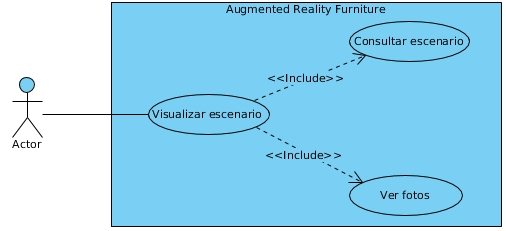
\includegraphics[width=12cm,height=6cm]{imagenes/analisis/visualizarEscenario.jpg}
	\caption{CU5 - Visualizar escenario.}
	\label{fig:analogo}
\end{figure}